\documentclass[10pt]{article}
\usepackage{tikz}
\usetikzlibrary{shapes.misc}
\usepackage[margin=0cm]{geometry}
\pagestyle{empty}
\tikzstyle{every node}=[cross out, draw, red]

\begin{document}

\vspace*{\fill}
\begin{center}
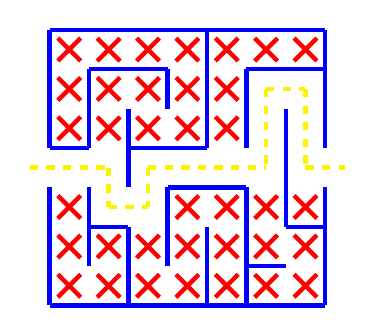
\begin{tikzpicture}[x=0.5cm, y=-0.5cm, ultra thick, blue]
% Walls
    \draw (0,0) -- (7,0);
    \draw (1,1) -- (3,1);
    \draw (5,1) -- (7,1);
    \draw (0,3) -- (1,3);
    \draw (2,3) -- (4,3);
    \draw (3,4) -- (5,4);
    \draw (1,5) -- (2,5);
    \draw (6,5) -- (7,5);
    \draw (5,6) -- (6,6);
    \draw (0,7) -- (7,7);
    \draw (0,0) -- (0,3);
    \draw (0,4) -- (0,7);
    \draw (1,1) -- (1,3);
    \draw (1,4) -- (1,6);
    \draw (2,2) -- (2,4);
    \draw (2,5) -- (2,7);
    \draw (3,1) -- (3,2);
    \draw (3,4) -- (3,6);
    \draw (4,0) -- (4,3);
    \draw (4,5) -- (4,7);
    \draw (5,1) -- (5,3);
    \draw (5,4) -- (5,7);
    \draw (6,2) -- (6,5);
    \draw (7,0) -- (7,3);
    \draw (7,4) -- (7,7);
%Pillars
%Inner points in accessible cul-de-sacs
    \node at (0.5,0.5) {};
    \node at (1.5,0.5) {};
    \node at (2.5,0.5) {};
    \node at (3.5,0.5) {};
    \node at (4.5,0.5) {};
    \node at (5.5,0.5) {};
    \node at (6.5,0.5) {};
    \node at (0.5,1.5) {};
    \node at (1.5,1.5) {};
    \node at (2.5,1.5) {};
    \node at (3.5,1.5) {};
    \node at (4.5,1.5) {};
    \node at (0.5,2.5) {};
    \node at (1.5,2.5) {};
    \node at (2.5,2.5) {};
    \node at (3.5,2.5) {};
    \node at (4.5,2.5) {};
    \node at (0.5,4.5) {};
    \node at (3.5,4.5) {};
    \node at (4.5,4.5) {};
    \node at (5.5,4.5) {};
    \node at (6.5,4.5) {};
    \node at (0.5,5.5) {};
    \node at (1.5,5.5) {};
    \node at (2.5,5.5) {};
    \node at (3.5,5.5) {};
    \node at (4.5,5.5) {};
    \node at (5.5,5.5) {};
    \node at (6.5,5.5) {};
    \node at (0.5,6.5) {};
    \node at (1.5,6.5) {};
    \node at (2.5,6.5) {};
    \node at (3.5,6.5) {};
    \node at (4.5,6.5) {};
    \node at (5.5,6.5) {};
    \node at (6.5,6.5) {};
%Entry-exit paths without intersections
    \draw[dashed, yellow] (5.5,1.5) -- (6.5,1.5);
    \draw[dashed, yellow] (-0.5,3.5) -- (1.5,3.5);
    \draw[dashed, yellow] (2.5,3.5) -- (5.5,3.5);
    \draw[dashed, yellow] (6.5,3.5) -- (7.5,3.5);
    \draw[dashed, yellow] (1.5,4.5) -- (2.5,4.5);
    \draw[dashed, yellow] (1.5,3.5) -- (1.5,4.5);
    \draw[dashed, yellow] (2.5,3.5) -- (2.5,4.5);
    \draw[dashed, yellow] (5.5,1.5) -- (5.5,3.5);
    \draw[dashed, yellow] (6.5,1.5) -- (6.5,3.5);
\end{tikzpicture}
\end{center}
\vspace*{\fill}

\end{document}
